%************************************************
\chapter{The Simulation}
\label{chapter:the_simulation}
%************************************************

It is imperative to understand that the \emph{simulation model} is not
the same as the model of mind that was previously described.  The
simulation model is an extension of the model of mind that includes a
mathematical description of a discrete ``state'' of the model in a
discrete time.  Neither the model of mind nor the simulation model
changes over time.  The simulation model therefore makes reference to
a discretely stepped state that is used to simulate the necessarily
separate, static model of mind.  The term ``simulation'' is thus used
as a general reference to the dynamic activity in Duration that
manipulates and steps the state of the simulation model.  In
describing the simulation model, it is important to not confuse the
dynamic activity of simulation with the model or the state of the
model, which are both static at any given point in time.  The term
``simulation'' is the only reference to activities in Duration.  This
distinction is necessary for the simulation model to not be limited to
simulating a specific kind of activity.

For example, consider a simulation of topological proof.  A
mathematician can ``simulate'' the rules of topological proof by first
seeing a static arrangement of symbols on paper.  These symbols can be
manipulated in the process of proving or disproving the initial
topological statement.  There is no existing logical or mathematical
formulation of the activities of topological proof.  I describe how a
symbolic state space can be added to the model of mind for the
purposes of simulation.  How exactly this simulation is done is left
until the next part, where the activity of simulation is assumed to be
computational.

The activities in Duration in the model of mind exist prior to their
symbolization, and since it is obviously not possible to refer to
something prior to symbolizing it, the assumption that these
activities have already been symbolized is necessary in order to
mathematically describe the state of the simulation model.  Defining
the simulation model requires a description in terms of symbols for
the ``undescribed activities in Duration.''  Each assumption made in
symbolizing the ongoing activities in Duration restricts the
simulation model from being a model of those assumptions because only
the symbolic result of those assumptions is available for the
simulation of the activity of reflection.

\section{Dynamic Activities as a Set}

\begin{figure}
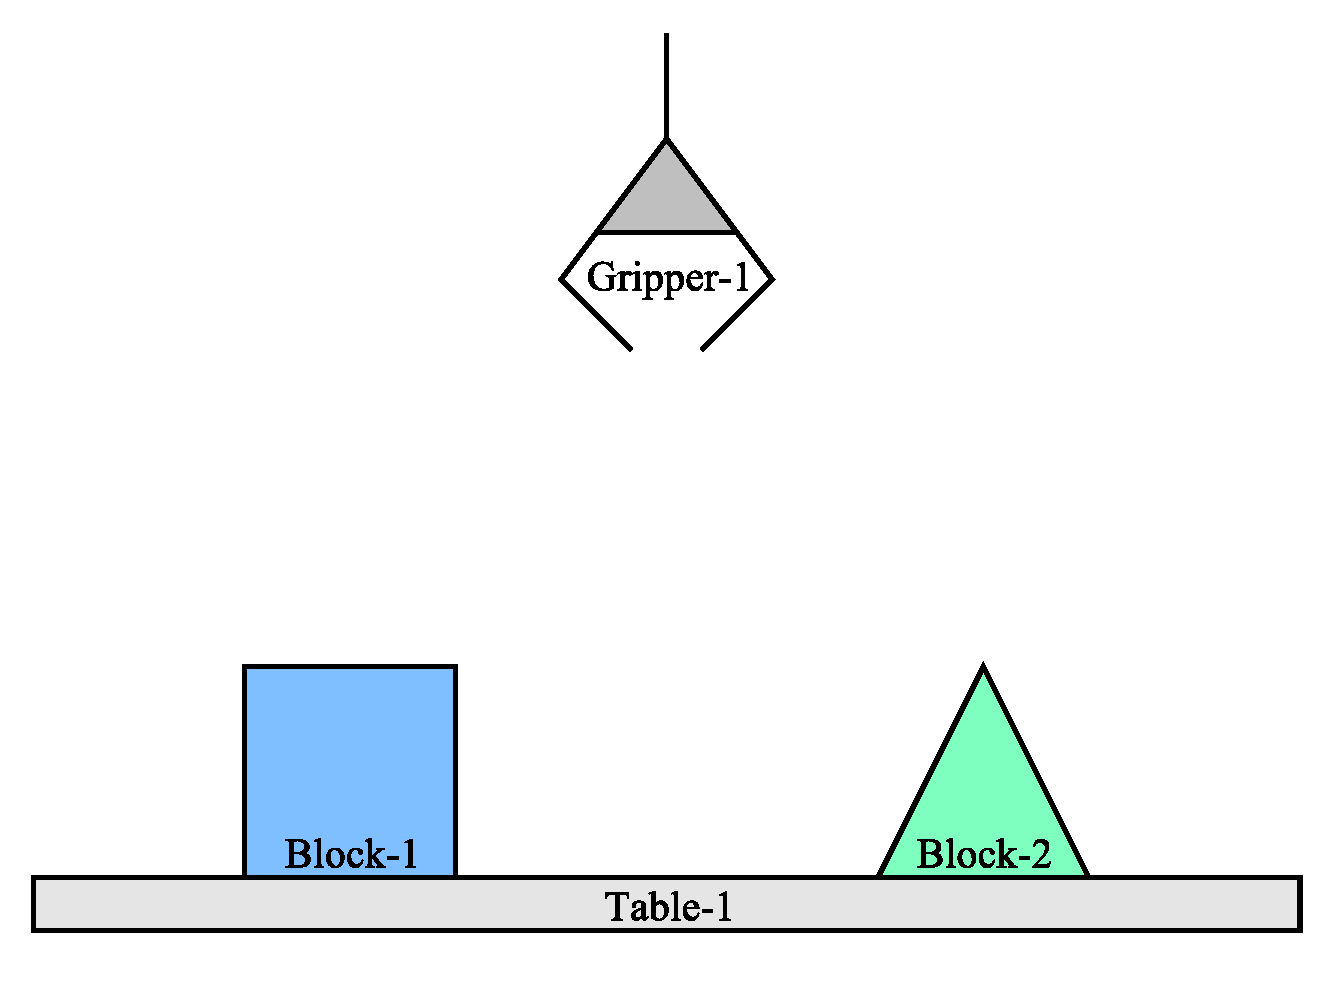
\includegraphics[width=10cm]{gfx/blocks_world_simulation}
\caption{An example for simulation.}
\label{figure:blocks_world_simulation}
\end{figure}

I will begin with one of the simplest mathematical models, a
\emph{set} of symbols, to model of the activities in Duration.  I will
first describe the simulation model as the mathematical set, X, the
activities of the state.  Here is an example of a possible
symbolization of the activities shown in
{\mbox{\autoref{figure:blocks_world_simulation}}}:
\begin{equation}
\label{equation:example_initial_state}
X =
  \left\{
    \begin{array}{l}
      \text{{\tt{Gripper-1}}}, \\
      \text{{\tt{Block-1}}}, \\
      \text{{\tt{Block-2}}}, \\
      \text{{\tt{Table-1}}} \\
      \text{{\tt{sitting-on}}}, \\
      \text{{\tt{being-above}}}, \\
      \text{{\tt{moving}}}, \\
      \text{{\tt{left}}}
    \end{array}
  \right\}
\end{equation}

\section{Representing Continuous Space as a Set of 3-Tuples}

The activities in Duration exist in a continuous Spatial arrangement
that is symbolized and ordered by the reflective thinking layers.  In
order to simulate this continuous homogenous Space, a discrete static
representation must be included in the state of the simulation model.
A 3-tuple can be used to represent the activity of a Spatial
relationship in the simulation.  Reconsidering the activities shown in
{\mbox{\autoref{figure:blocks_world_simulation}}}, the state could be
represented by the set of 3-tuples shown in
{\mbox{\autoref{equation:example_stricly_ordered_set_initial_state}}}.
\begin{equation}
\label{equation:example_stricly_ordered_set_initial_state}
\text{triples}(S) =
  \left\{
    \begin{array}{l}
      (\text{\tt{Block-1}},   ~\text{\tt{sitting-on}},  ~\text{\tt{Table-1}}), \\
      (\text{\tt{Block-2}},   ~\text{\tt{sitting-on}},  ~\text{\tt{Table-1}}), \\
      (\text{\tt{Gripper-1}}, ~\text{\tt{being-above}}, ~\text{\tt{Table-1}}), \\
      (\text{\tt{Gripper-1}}, ~\text{\tt{moving}},      ~\text{\tt{left}})
    \end{array}
  \right\}
\end{equation}

\section{A Graph Representation}

A set of 3-tuples can be thought of as a graph of nodes with labelled
edges.  Because the graph provides a clear notation for referring to
types of Spatial arrangements of activities, a modified notation
originally from {\mbox{\cite{messmer:1995}}} is used to define a
labelled graph in {\mbox{Definition~\ref{definition:graph_first}}} and
a labelled subgraph in
{\mbox{Definition~\ref{definition:graph_last}}}.

\begin{definition}
\label{definition:graph_first}
\emph{
A graph $G$ is the 3-tuple $(V, ~E, ~\mu)$, where
\begin{itemize}
\item $V$ is the set of vertices,
\item $E ~{\subseteq}~ V ~{\times}~ V$ is the set of edges,
\item $\mu : E \mapsto \{\ell_E\}$ is a function assigning a set of labels to each edge.
\end{itemize}
}\end{definition} \noindent In this definition, the edges are
directed, i.e. there is an edge from $v_1$ to $v_2$ if $(v_1,
v_2){\in}E$.  The empty graph, i.e. the graph with an empty set of
vertices will be denoted by $\emptyset$.  The union of the set of
vertices with the set of labels referred to by $\mu$ will be sometimes
be referred to with a dot notation, $\mathring{G}=V {\cup} \ell_E$.

\begin{definition}
\label{definition:graph_last}
\emph{ Given a graph $G = (V, E, \mu)$, a \emph{subgraph} of $G$ is a
  graph $G_s = (V_s, E_s, \mu_s)$ such that
\begin{enumerate}
\item $V_s ~{\subseteq}~ V$
\item $E_s ~{\subseteq}~ V_s {\times} V_s$,
\item $\mu_s$ is the restriction of $\mu$, i.e.
\begin{align*}
\mu_s(\overrightarrow{e}) &\subseteq
   {\left\{
      \begin{array}{ll}
        \mu(\overrightarrow{e})     & \text{if }\overrightarrow{e} {\in} E_s \\
        \text{undefined} & \text{otherwise}
      \end{array}
    \right.}
\end{align*}
\end{enumerate}
}\end{definition} \noindent From this definition it is easy to see
that, given a graph $G$, any subset of its vertices and an included
subset of its edges uniquely defines a subgraph of $G$.  The notation
$G_s ~{\subseteq}~ G$ is used to indicate that $G_s$ is a subgraph of
$G$.

\section{Representing Continuous Space as a Graph}

{\mbox{\autoref{figure:simulation_example_state}}} shows the example
simulation state state, initially presented in
{\mbox{\autoref{equation:example_stricly_ordered_set_initial_state}}},
as a set of 3-tuples, represented as a graph.  Graph notation will be
used to describe the activities in Duration and continuous Space,
which exist before they are symbolized and discretely ordered by the
$\text{reflective}^1$ layer.  The simulation model state space, $S$,
is defined to be a graph in
{\mbox{Equations~\ref{equation:define_graph_state_first}}}
{\mbox{through~\ref{equation:define_graph_state_last}}}.
\begin{align}
\label{equation:define_graph_state_first}
       S &= (S_V, ~S_E, ~S_\mu) \\
     S_V &= {\left\{
               \begin{array}{l}
                 \text{\tt{Gripper-1}}, \\
                 \text{\tt{Block-1}}, \\
                 \text{\tt{Block-2}}, \\
                 \text{\tt{Table-1}}, \\
                 \text{\tt{left}}
               \end{array}
             \right\}} \\
     S_E &= {\left\{
               \begin{array}{l}
                 (\text{\tt{Gripper-1}}, \text{\tt{Table-1}}), \\
                 (\text{\tt{Block-1}}, \text{\tt{Table-1}}), \\
                 (\text{\tt{Block-2}}, \text{\tt{Table-1}}), \\
                 (\text{\tt{Gripper-1}}, \text{\tt{left}})
               \end{array}
             \right\}} \\
\label{equation:define_graph_state_last}
S_\mu(\overrightarrow{e}) &=
  {\left\{
     \begin{array}{ll}
       \{\text{\tt{being-above}}\} & \text{if }\overrightarrow{e} = (\text{\tt{Gripper-1}}, \text{\tt{Table-1}}) \\
       \{\text{\tt{sitting-on}}\}  & \text{if }\overrightarrow{e} = (\text{\tt{Block-1}}, \text{\tt{Table-1}}) ~{\vee}~ \\
                                   & \text{~~ }\overrightarrow{e} = (\text{\tt{Block-2}}, \text{\tt{Table-1}}) \\
       \{\text{\tt{moving}}\}      & \text{if }\overrightarrow{e} = (\text{\tt{Gripper-1}}, \text{\tt{left}}) \\
       \text{undefined} & \text{otherwise}
     \end{array}
   \right.}
\end{align}
\begin{figure}
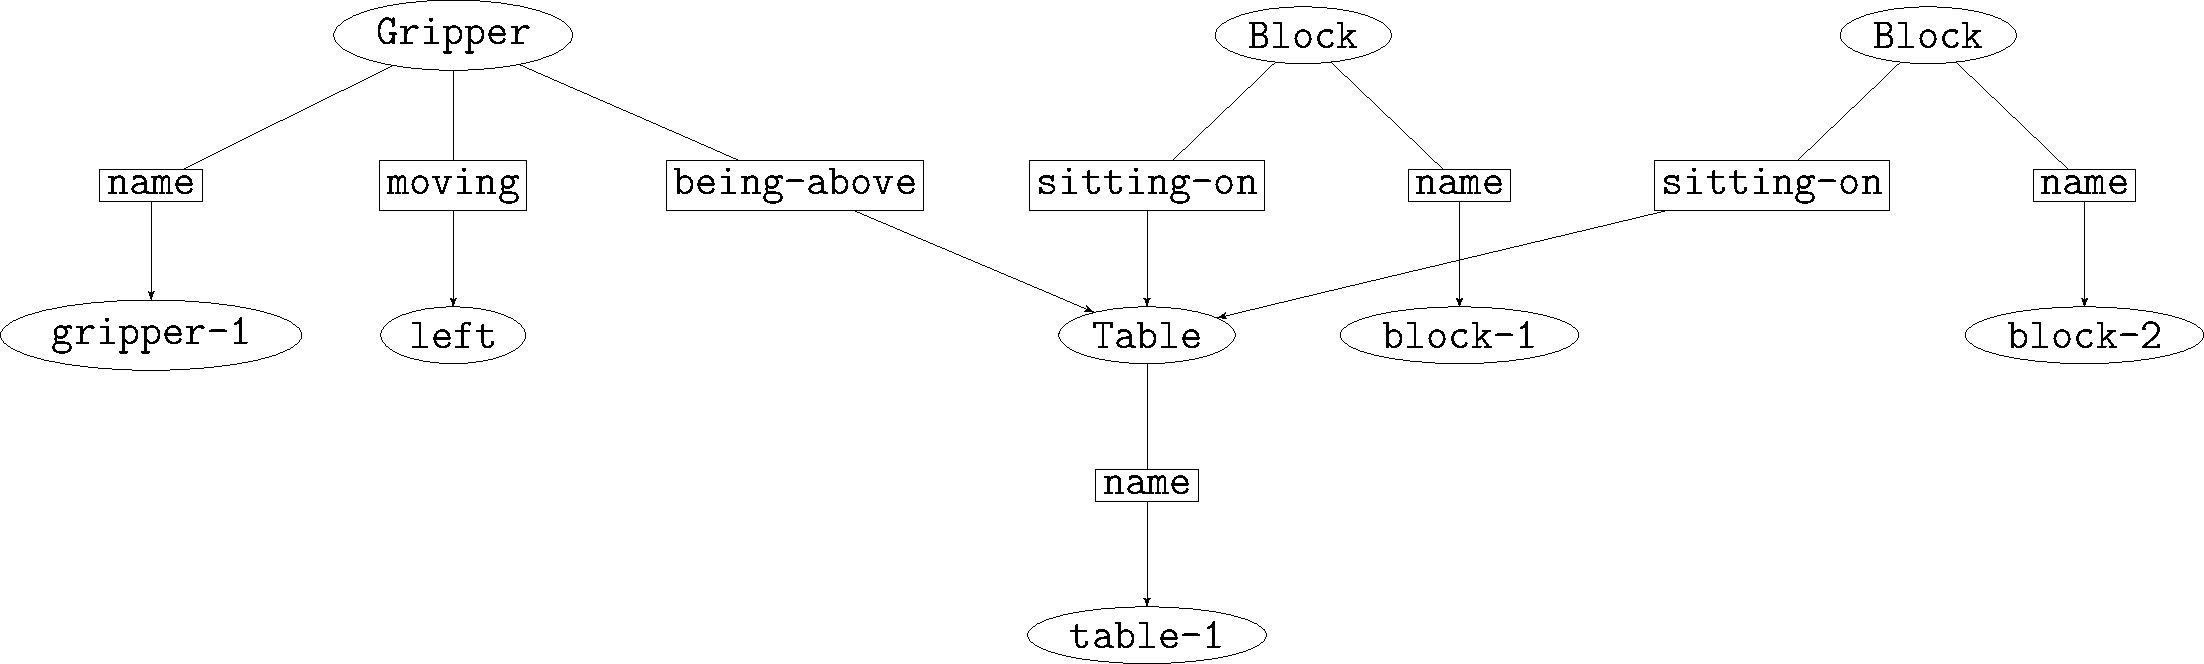
\includegraphics[width=10cm]{gfx/simulation_example_state}
\caption[A labelled graph representation of a state space.]{A labelled graph representation of a state space, where circles represent nodes, and squares represent edges.}
\label{figure:simulation_example_state}
\end{figure}

\section{Dot Notation for Graph-based Frame Objects}

Sometimes it is useful to refer to parts of a graph by considering
nodes in the graph to represent frame objects that have slotted
relationships with other frame objects.  Thus, I use a dot notation to
refer to the set of nodes that are connected to a given node, $v_1$,
through a given edge label, $\ell_e$, as defined in
{\mbox{\autoref{equation:frame_dot_notation}}}.
\begin{equation}
\label{equation:frame_dot_notation}
v_1.\ell_e = \{v_2 ~:~ (v_1, v_2) \in S_E \wedge \ell_e \in \mu[(v_1, v_2)]\}
\end{equation}

\section{Frame Object Types}

In order to allow for object-oriented types of frames in the
simulation state, I will use the edge label ``{\tt{type}}''.  For
example, {\mbox{\autoref{equation:frame_type_symbol}}} states that
$x^*$ is a symbolic type of activity:
\begin{equation}
\label{equation:frame_type_symbol}
x^*.\text{\tt{type}} = \{\text{\tt{symbol}}\}
\end{equation}
Because there are a number of different frame object types that are
created by the model, the simulation state includes a representation
for a simple ontology for these frame types.  I use the edge label
``{\tt{parent}}'' to represent the inheritance structure of a frame
type.  For example, {\mbox{\autoref{equation:goal_parent_symbol}}}
defines that the object type ``{\tt{goal}}'' is a type of
``{\tt{symbol}}'' frame object:
\begin{equation}
\label{equation:goal_parent_symbol}
  \text{\tt{goal}}.\text{\tt{parent}} = \{\text{\tt{symbol}}\}
\end{equation}
Further, types of objects are explicitly represented as type objects
as in {\mbox{\autoref{equation:frame_type_type}}}.
\begin{align}
\label{equation:frame_type_type}
  \text{\tt{symbol}}.\text{\tt{type}} &= \{\text{\tt{type}}\} \\
    \text{\tt{goal}}.\text{\tt{type}} &= \{\text{\tt{type}}\}
\end{align}
The inheritance structure of some basic frame object types in the
simulation model are shown in
{\mbox{\autoref{figure:basic_frame_object_types}}}.
\begin{figure}
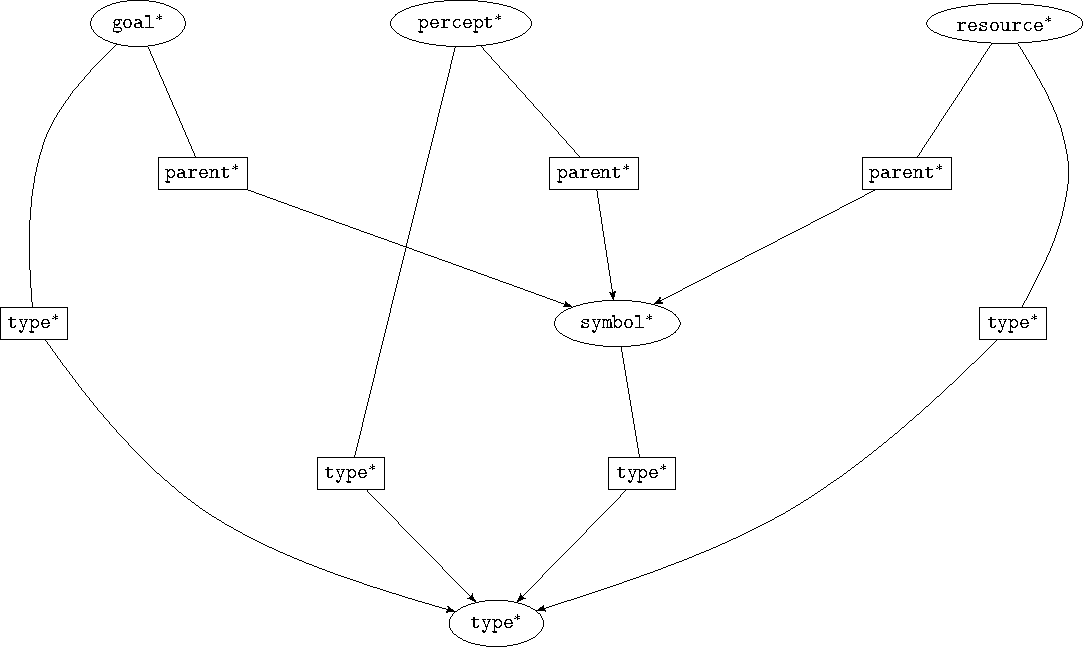
\includegraphics[width=10cm]{gfx/basic_frame_object_types}
\caption{Basic frame object types.}
\label{figure:basic_frame_object_types}
\end{figure}

\section{Simulated Existence}

Activities in continuous Space actually exist.  Once we have
considered the activities in Duration to be the set of symbols, $S$,
we have assumed static representations for the actual dynamic.  The
dynamic does not have terms to help us in representing.  Therefore,
the question of existence becomes a question of whether or not a
symbol is in the set that is the current state of the simulation, $S$.
Equation~\ref{equation:exists} shows a definition of {\tt exists},
defined as the subgraph relationship between any state, $x$,
represented as a labelled graph, and the currently simulated state
graph, $S$:
\begin{equation}
\label{equation:exists}
\text{exists}(x) \longleftrightarrow x ~{\subseteq}~ S
\end{equation}

\section{Representing Symbolic Reference}

In order to describe symbolization, a representation for a simulated
symbol must be defined.  A symbol is the most interesting object in
the model because it functions as a static reference to the dynamic,
while being fundamentally dynamic itself.  There are two primary
features of a symbolic reference:
\begin{itemize}
\item A symbol functions as a static reference and, thus, can be
  ordered in Spatial arrangements that function as static orderings.
\item A symbol is fundamentally dynamic and, thus, exists as dynamic
  activities in a referential dynamic continuous Spatial relationship
  with other dynamic activities in Duration.
\end{itemize}
A symbol is actively maintained in Duration, so the existence of a
simulated symbol in the simulation model would need to be added to the
set of all simulated activities in Duration.  The symbol*, $x^*$, has
a referent, $\rho(x^*)$, a subgraph of the simulated activities in
Duration, $S$, in Equations~\ref{equation:symbolization_first}
and~\ref{equation:symbolization_last}:
\begin{align}
\label{equation:symbolization_first}
                                       X^* &\equiv \text{\emph{The set of symbols*}} \\
                                       x^* &\in X^* \\
                                 \rho(x^*) &\subseteq S \\
 \forall_{x{\in}\mathring{S}} x{\in}\rho(x^*) &\rightarrow (x^*, x) \subseteq S_E \wedge \text{\tt{referent}} \in S_\mu((x^*, x))
\label{equation:symbolization_last}
\end{align}

Symbols are defined in terms of their referents.  If an activity does
not have a symbolic referent, then it is not a symbolic activity.  The
following equation expresses the logical definition that symbols
cannot have empty referent sets:
\begin{equation*}
\rho(x^*) \neq \emptyset
\end{equation*}

\section{Representing Static Space}

In order to refer to a simulated ordered static Spatial relationship,
I will use an astrisk superscript, a Spatial* relationship.
Therefore, symbols* are arranged in Space*.  Using this asterisk
notation, it should be easier to keep track of what parts of the
simulation are of the actual dynamic and which are of the static, the
asterisk referring to the static components.

The activity of maintaining a static Spatial relationship, $e^*$,
statically arranges symbols*, $X^*$.
Equations~\ref{equation:define_space_activity_first}
through~\ref{equation:define_space_activity_last} define how symbols
are statically Spatially arranged, $e^*$:
\begin{align}
\label{equation:define_space_activity_first}
        {S_E}^* &= \left\{\overrightarrow{e} : \overrightarrow{e}{\in}S_E \wedge (v_1, v_2) {\in} {X^*}^2\right\}, ~\text{\emph{Static Spatial relationships}} \\
      \overrightarrow{e}^* &\in {S_E}^* \\
\label{equation:define_space_activity_last}
      \overrightarrow{e}^* &= (v_1^*, ~v_2^*)
\end{align}
Spatial relationships can refer to other Spatial relationships from
the same layer because the activity of the Spatial relationship is in
the layer below the symbols that it arranges, so one arrangement can
be symbolized and referred to by another arrangement from the same
layer.

\section{Representing a Transition}

In order for a thinking activity in the $\text{reflective}^1$ layer to
refer to types of Spatial arrangements, must also be statically
symbolic as well.  In the graph representation this means that not
only do the vertices of an edge need to be static symbols but also, in
order for this Space to be accessible to thinking, the edge labels
need to be static symbols as well.

\begin{align}
\text{\tt{future}}^* &\in \mu((x^*, x.\text{future}^*)) \\
  \text{\tt{past}}^* &\in \mu((x^*, x.\text{past}^*)) 
\end{align}



\section{Representing Spatial Reflection}

Spatial* arrangements of symbols* can be represented as a graph* in or
above the simulated $\text{reflective}^2$ layer, where Spatial*
relationship edge activities in the $\text{reflective}^0$ layer order
symbolic vertex activities in the $\text{reflective}^1$ layer.  The
$\text{reflective}^2$ layer can symbolize these edge and vertex
activities, which provides the $\text{reflective}^2$ layer symbolic
labels for referring to useful parts of these graph structures in the
layers below.

\begin{definition}
\label{definition:graph_first}
\emph{
A graph $G$ is the 4-tuple $(V, ~E, ~\mu, ~\nu)$, where
\begin{itemize}
\item $V$ is the set of vertices,
\item $E ~{\subseteq}~ V ~{\times}~ V$ is the set of edges,
\item $\mu : V \mapsto \ell_V$ is a function assigning a label to each vertex,
\item $\nu : E \mapsto {\ell_E}^*$ is a function assigning a set of labels to each edge.
\end{itemize}
}\end{definition} \noindent





\section{Tautological Symbolic Reference}

{\mbox{Equations~\ref{equation:tautological_reference_first}}}
{\mbox{through~\ref{equation:tautological_reference_last}}} give an
example of a symbol*, $x^*$, that tautologically references its own
symbolization activity:
\begin{align}
\label{equation:tautological_reference_first}
\rho(x^*) &= (V_x, ~E_x, ~\mu_x, ~\nu_x) \\
 V_{x^*}   &= \{v_1\} \\
 E_{x^*}   &= \emptyset \\
 \mu_{x^*} &= v : \{v_1\} ~{\mapsto}~ \{x^*\} \\
\label{equation:tautological_reference_last}
            \nu_{x^*} &= e : \emptyset ~{\mapsto}~ \emptyset
\end{align}
Tautological references are meaningless.  In a model that is
symbolizing and perceiving the world in terms of symbols, tautological
symbolic references always have the potential for being active
perceptions because the existence of a tautological symbol implies
that its referent, itself, is active.  When symbols are used for
perception, tautological references are at best distracting and at
worst render a model meaningless.

Because a tautological reference removes all utility from symbols* in
the simulation model, it is important that avoiding tautological
references is the default behavior.  In order to easily avoid
tautological references, I define an ordering for symbolic references
that keeps references from ever becoming purely tautological.

\section{Representing Layers of Continuous Spaces of Dynamic Activity}

In order to avoid tautological symbolic references, I have divided the
model into layers that order symbolic activities and references.  To
simulate the $\text{reflective}^n$ layers of activity in the model, I
must define the simulation state graph, $S$, to be composed of
disjoint subgraphs, one for each reflective layer.
Equations~\ref{equation:layers_of_sets_first}
through~\ref{equation:layers_of_sets_last} give a definition of the
disjoint set of layers, $\mathbf{L}$, stating that the union of all
layers of activity is equal to the simulation state graph, $S$:
\begin{align}
\label{equation:layers_of_sets_first}
                            L_i &= \text{\emph{Spatial arrangement of activities in the} }\text{reflective}^i\text{ \emph{layer}} \\
                     \mathbf{L} &= \{L_0, ~L_1, ~L_2, ~...~ \} \\
\label{equation:layers_are_mututally_exclusive}
\forall_{A,B{\in}{\mathbf{L}}} ~ (A &= B ~{\vee}~ A{\cup}B = {\emptyset}) \\
\label{equation:layers_of_sets_last}
                              S &= \bigcup_{A{\in}\mathbf{L}}{A}
\end{align}
{\mbox{\autoref{equation:layers_are_mututally_exclusive}}} defines the
mutual exclusivity of layer activities.  Using these reflective layer
definitions, I define an ordering of symbol* references that prevents
symbols from every having tautological references.  Finally, the
purpose of creating layers in the first place, avoiding purely
tautological symbolic references,
equation~\ref{equation:layered_symbol_references} defines that a
symbol may only refer to activities in the layers below its own layer
of activity:
\begin{equation}
\label{equation:layered_symbol_references}
\forall_{x^* \in L_i}~\rho(x^*) \subseteq \bigcup_{k=0}^{i-1}{L_k}
\end{equation}

\section{No Symbols* in Layer Zero}

Equations~\ref{equation:no_symbols_in_layer_zero_first}
through~\ref{equation:no_symbols_in_layer_zero_last} derive that a
symbol* cannot actively exist in the simulated reflective layer zero,
$L_0$.  Equation~\ref{equation:no_symbols_in_layer_zero_first} derives
from the layered symbolic references equation,
Equation~\ref{equation:layered_symbol_references}.
\begin{align}
\label{equation:no_symbols_in_layer_zero_first}
\forall_{x^* \in L_i}~\rho(x^*) &\subseteq \bigcup_{k=0}^{i-1}{L_k}, \text{~given~} i=0 \\
\forall_{x^* \in L_0}~\rho(x^*) &\subseteq \emptyset \\
\label{equation:no_symbols_in_layer_zero_last}
\forall_{x^* \in L_0}~\rho(x^*) &= \emptyset
\end{align}







\section{leftovers...}

\section{Simulation States}

At any given point in the simulation, the state, $S$, is static, but
the simulation can have different static states at different time
steps, $n$, giving a number of static states, $S[n]$.  The simulation
process is a discrete stepwise activity.  The simulation step is the
dynamic activity that is not part of the state, $S$, of the simulation
model.  I will now describe a notation for referring to the different
states that result from a simulation process.

Equations~\ref{equation:simulate_first}
and~\ref{equation:simulate_last} show a notation for referring to the
state of a simulation after a number of simulation steps, $n$.
\begin{align}
\label{equation:simulate_first}
S[0] &= \text{\emph{The Initial State}} \\
\label{equation:simulate_last}
S[n] &= \text{\emph{simulate}}~S[n-1]
\end{align}
Equation~\ref{equation:simulate_first} defines $S[0]$ to be
the initial representation of the activities in Duration that are
being simulated; an example of the initial state was given previously
in Equation~\ref{equation:example_initial_state}.
Equation~\ref{equation:simulate_last} introduces an explicit reference
to the activity of simulation with the symbol ``simulate.''  Because I
have not yet defined this activity, these equations still have a
reference to the actual dynamic activity of simulation.  I use this
notation to discuss how the state, $S$, changes during the
actual process of simulation.  I will use the notation in
Equation~\ref{equation:simulate_n_steps} to refer to the state of the
simulation after $n$ actual steps of simulation activity:
\begin{equation}
\label{equation:simulate_n_steps}
S[n] = \text{\emph{simulate}}^n~S[0]
\end{equation}

\section{Representing the Transition}

Equations~\ref{equation:define_transition_activity_first}
through~\ref{equation:define_transition_activity_future} define a
transition, $t_i$:
\begin{align}
\label{equation:define_transition_activity_first}
               t_i &= \text{\emph{Transition activity in the} reflective}^i\text{\emph{ layer}} \\
               t_i &\in L_i \\
\label{equation:define_transition_activity_past}
  \text{past}(t_i, n) &\in X_{i+1}^* \\
\label{equation:define_transition_activity_future}
\text{future}(t_i, n) &\in X_{i+1}^*
\end{align}

\section{Representing the Hypothesis}

Equations~\ref{equation:define_hypothesis_activity_first}
through~\ref{equation:define_hypothesis_activity_result} define a
hypothesis, $h_i$:
\begin{align}
\label{equation:define_hypothesis_activity_first}
                  h_i &= \text{\emph{Hypothesis activity in the} reflective}^i\text{\emph{ layer}} \\
                  h_i &\in L_i \\
\label{equation:define_hypothesis_activity_cause}
    \text{cause}(h_i) &\in X_{i+1}^* \\
\label{equation:define_hypothesis_activity_necessity}
\text{necessity}(h_i) &\in X_{i+1}^* \\
\label{equation:define_hypothesis_activity_result}
   \text{result}(h_i) &\in X_{i+1}^*
\end{align}

\section{Representing Existence and Non-existence}

When the $\text{reflective}^1$ layer symbolizes physical activities, a
causal hypothesis can be created in the $\text{reflective}^2$ layer
that puts a reference to the ``non-existence'' of the symbol activity
in the past slot and the ``existence'' of the symbol in the future
slot.  The present cause can be any of the current activities in
either the $\text{reflective}^0$ or $\text{reflective}^1$ layers.
{\mbox{Equations~\ref{equation:define_creation_activity_first}}}
{\mbox{through~\ref{equation:define_creation_activity_existence}}}
show a representation for the simulation of the creation activity that
creates the existence of an activity in the layer below from the
``non-existence'' of the activity.
\begin{align}
\label{equation:define_creation_activity_first}
                      c_i &= \text{\emph{Creation activity in the} reflective}^i\text{\emph{ layer}} \\
                      c_i &\in L_i \\
\label{equation:define_creation_activity_cause}
        \text{cause}(c_i) &\in X_{i+1}^* \\
\label{equation:define_creation_activity_non_existence}
\text{non-existence}(c_i) &\in X_{i+1}^* \\
\label{equation:define_creation_activity_existence}
    \text{existence}(c_i) &\in X_{i+1}^*
\end{align}

\section{Representing Knowledge of Symbolic Existence}


\section{Simulating Goals}

Activities in Duration can be symbolized as goals.  The symbolization
of a goal in the $\text{reflective}^i$ layer can be simulated by the
symbolic simulated activity, $g_i$.

\section{Simulating the Transframe}

Equations~\ref{equation:define_transframe_activity_first}
through~\ref{equation:define_transframe_activity_remove} define a
transframe, $\text{trans}_i$:
\begin{align}
\label{equation:define_transframe_activity_first}
                  \text{trans}_i &= \text{\emph{Transframe activity in the} reflective}^i\text{\emph{ layer}} \\
                  \text{trans}_i &\in L_i \\
\label{equation:define_transframe_activity_add}
   \text{add}(\text{trans}_i) &\in X_{i+1}^* \\
\label{equation:define_transframe_activity_remove}
\text{remove}(\text{trans}_i) &\in X_{i+1}^*
\end{align}


% Original definition of a graph as a 4-tuple with labelled nodes and edges

%\begin{definition}
%\label{definition:graph_first}
%\emph{
%A graph $G$ is the 4-tuple $(V, ~E, ~\mu, ~\nu)$, where
%\begin{itemize}
%\item $V$ is the set of vertices,
%\item $E ~{\subseteq}~ V ~{\times}~ V$ is the set of edges,
%\item $\mu : V \mapsto \ell_V$ is a function assigning a label to each vertex,
%\item $\nu : E \mapsto \{\ell_E\}$ is a function assigning a set of labels to each edge.
%\end{itemize}
%}\end{definition} \noindent In this definition, the edges are
%directed, i.e. there is an edge from $v_1$ to $v_2$ if $(v_1,
%v_2){\in}E$.  The empty graph, i.e. the graph with an empty set of
%vertices will be denoted by $\emptyset$.  The union of the sets of
%labels referred to by $\mu$ and $\nu$ will be sometimes be referred to
%with a dot notation, $\mathring{G}=\ell_V {\cup} \ell_E$.
%
%\begin{definition}
%\label{definition:graph_last}
%\emph{ Given a graph $G = (V, e, \mu, \nu)$, a \emph{subgraph} of $G$
%  is a graph $G_s = (V_s, e_s, \mu_s, \nu_s)$ such that
%\begin{enumerate}
%\item $V_s ~{\subseteq}~ V$
%\item $E_s ~{\subseteq}~ V_s {\times} V_s$,
%\item $\mu_s$ and $\nu_s$ are the restrictions of $\mu$ and $\nu$,
%  respectively, i.e.
%\begin{align*}
%\mu_s(v) &=         {\left\{
%                       \begin{array}{ll}
%                         \mu(v)           & \text{if }v {\in} V_s \\
%                         \text{undefined} & \text{otherwise}
%                       \end{array}
%                     \right.} \\
%\nu_s(e) &\subseteq {\left\{
%                       \begin{array}{ll}
%                        \nu(e)           & \text{if }e {\in} E_s \\
%                        \text{undefined} & \text{otherwise}
%                       \end{array}
%                     \right.}
%\end{align*}
%\end{enumerate}
%}\end{definition}



%\section{Simulating the Plan}
%


%\section{State Transitions (should be rewritten in simulation objects)} 

%\autoref{figure:blocks_world_gripper_over_block} shows an example of
%the next state of the simulation, $S[1]$.
%Equation~\ref{equation:example_next_state} gives an example
%description of the next state of the simulation model:
%\begin{figure}[bth]
%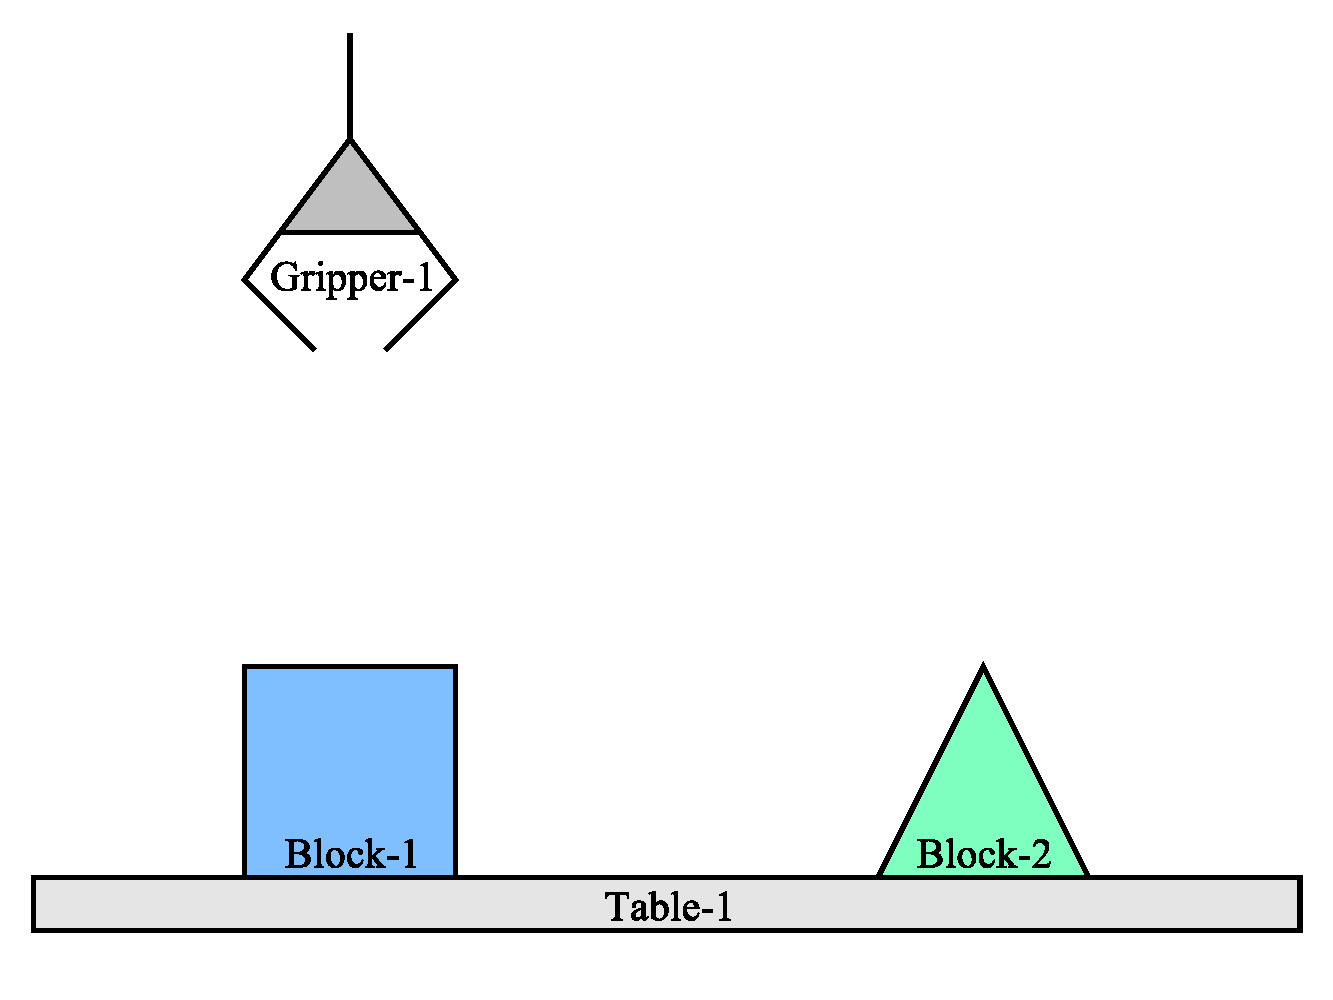
\includegraphics[width=10cm]{gfx/blocks_world_gripper_over_block}
%\caption{An example future state of simulation.}
%\label{figure:blocks_world_gripper_over_block}
%\end{figure}
%\begin{equation}
%\label{equation:example_next_state}
%S[1] =
%  \left\{
%    \begin{array}{l}
%      \text{{\tt Block-1-sitting-on-Table-1}}, \\
%      \text{{\tt Block-2-sitting-on-Table-1}}, \\
%      \text{{\tt Gripper-1-hovering-above-Table-1}}, \\
%      \text{{\tt Gripper-1-hovering-above-Block-1}}
%    \end{array}
%  \right\}
%\end{equation}
%
%Now, in order to begin to describe the activity of simulation, we must
%explicitly represent the transition, $T$, from one state to another.
%I refer to the resulting change to the state of the simulation as a
%\emph{state transition}.  The transition, $T[n]$, consists of two sets
%that keep track of changes, the \emph{add} set and the \emph{remove}
%set, as shown in Equation~\ref{equation:state_transition}:
%\begin{equation}
%\label{equation:state_transition}
%T[n] = \{T_\text{add}[n], ~T_\text{remove}[n]\}
%\end{equation}
%Equations~\ref{equation:predictive_state_transition}
%through~\ref{equation:transframe_last} give a definition of the
%transition, $T[n]$, in terms of the states, $S[n]$ and
%$S[n+1]$:
%\begin{align}
%\label{equation:predictive_state_transition}
%          S[n+1] & = S[n] ~{\cup}~ T_\text{add}[n] ~{\setminus}~ T_\text{remove}[n] \\
%         T_\text{remove}[n] & ~{\subseteq}~ S[n] \\
%         T_\text{remove}[n] & ~{\not\subseteq}~ S[n+1] \\
%            T_\text{add}[n] & ~{\subseteq}~ S[n+1] \\
%\label{equation:transframe_last}
%            T_\text{add}[n] & ~{\not\subseteq}~ S[n]
%\end{align}
%Equations~\ref{equation:state_transition_first}
%and~\ref{equation:state_transition_last} give the state transition,
%$T[n]$, for every step of the simulation:
%\begin{align}
%  \label{equation:state_transition_first}
%     T_\text{add}[n] &= S[n+1] ~{\setminus}~ S[n] \\
%  \label{equation:state_transition_last}
%  T_\text{remove}[n] &= S[n]   ~{\setminus}~ S[n+1]
%\end{align}
%Equation~\ref{equation:predictive_state_transition} shows the
%predictive potential for knowing the transition, $T[n]$, given the
%current state, $S[n]$.  Of course, $T[n]$ is defined in
%terms of $S[n]$ \emph{and} $S[n+1]$, so any
%predictive potential for
%Equation~\ref{equation:predictive_state_transition} is purely
%hypothetical.

